\newpage
\section{Results and sensitivity analysis}\label{results}
This section presents the most relevant results of the proposed case study. Section \ref{res:overview} compares the results of the district heating or heat-pump-based heat supply in the different scenarios. Section \ref{res:district_heating} puts the focus on the district heating option results in the \textit{Directed Transition} scenario and Section \ref{res:heat_pump} on the implementation of a heat pump system in the \textit{Societal Commitment} scenario. Latter highlights the impact of passive retrofitting measures on the feasibility of the model when implementing a heat pump in the old building and subsidization strategy and presents a sensitivity analysis regarding the total heat demand of the building as a parameter. Finally, Section \ref{res:co2_shares} presents the results in the case of a CO\textsubscript{2} pricing cost allocation between the landlord as the building's owner and the tenants. 

\subsection{Objective value and results comparison}\label{res:overview}
Table \ref{tab:objective} shows a comparison of the obtained objective values for district heating (DH) and heat pump implementation in the different scenarios. 

\definecolor{Gray}{gray}{0.95}
\begin{table}[h]
	\centering
	\resizebox{\columnwidth}{!}{
		\renewcommand{\arraystretch}{1.35}
		\begin{tabular}{lcccccc}
			\toprule 
			& \multicolumn{3}{c}{District heating (DH)} & \multicolumn{3}{c}{Heat pump (HP)}\\
			\cmidrule(lr){2-4}\cmidrule(lr){5-7}
			 & DT & GD & LD & SC & GD& LD\\
			 \cmidrule(lr){2-2}\cmidrule(lr){3-3}\cmidrule(lr){4-4}\cmidrule(lr){5-5}\cmidrule(lr){6-6}\cmidrule(lr){7-7}
			Objective value & (\SI{1.5}{\degreeCelsius}) & (\SI{2.0}{\degreeCelsius}) & (-) & (\SI{1.5}{\degreeCelsius}) &  (\SI{2.0}{\degreeCelsius}) & (-)\\
			\hline
			Absolute in thous. \SI{}{EUR} & \SI{211.4}{} & \SI{195.5}{} & \cellcolor{Gray}\SI{190.1}{} & \textit{infeasible} & \textit{infeasible} & \SI{351.5}{}\\
			Rel. change in \% of LD (DH) & \SI{11.2}{} & \SI{2.6}{} & - &  & & \SI{82.6}{}\\ 
			\bottomrule
	\end{tabular}}
	\caption{Comparison of objective value results for the different heating system alternatives and scenarios}
	\label{tab:objective}
\end{table}

In particular, two important aspects can be obtained while studying this table. The values across the three district heating cases are relatively stable and are within \SI{11.2}{\%}. In addition, the heat pump implementation in the two decarbonization scenarios \textit{Societal Commitment} and \textit{Gradual Development} is infeasible. In this context, only the low CO\textsubscript{2} price development provides a solution for the heat pump but with a significantly higher value compared to the scenario with the lowest value (+\SI{82.6}{\%} compared with the lowest value).\vspace{0.5cm}

Figure \ref{fig:npv_comparison} shows the subsidization from the governance for the different technologies and scenarios. Note that the landlord's rent-related revenues (orange bar) are an implicit subsidy. Hence, the objective values from above are equal to the sum of the tenants' heating costs subsidy (purple bar) and the landlord's investment grant (blue bar). 

\begin{figure}[h]
	\centering
	\includegraphics[width=0.7\linewidth]{figures/4_Results/fig_npv_comparison/net_present_value.eps}
	\caption{Comparison of subsidiziation from the governance for the landlord and the tenants for district heating (DH) and heat pump (HP) implementation in the different scenarios}
	\label{fig:npv_comparison}
\end{figure}

\subsection{District heating in the Directed Transition scenario}\label{res:district_heating}
This section presents the results of the district heating implementation in the \textit{Directed Transition} scenario in detail. Figure \ref{fig:dt+dh} shows the revenues and net present value of the landlord and a single tenant within the time horizon $2025$ to $2040$. The subfigure at the top left shows the revenues of the landlord consisting of the overnight investment costs (light blue), investment grant (blue), and rent-related revenues (yellow). Note that later represent the additional rent-related revenues based on the modernization of the building regarding the newly installed sustainable heating system alternative. The subfigure at the bottom left shows the development of the landlord's net present value. Thereby, it is shown that the investment achieves a net present value equal to zero at the end of the time horizon in 2040. The two subfigures to the right illustrate the tenant's revenues (top) and net present value (bottom). The tenant gets subsidy payments from the governance between 2025 and 2030. Thus, the tenant's net present value achieves the same value as in the reference case. The reference case considers constant remaining rent- and heat-related costs for the tenant based on the initial rent, gas, and CO\textsubscript{2} as in 2025. In the years 2025 to 2029, the subsidy payments exceed the heating costs of the tenant. Note that the tenant already pays a higher rent charge to the landlord within the same period (see the yellow bars in the top left subfigure).

\begin{figure}[h]
	\centering
	\includegraphics[width=1\linewidth]{figures/4_Results/fig_DT_DH/detail.eps}
	\caption{Development of the landlord's and tenant's economic viability of the district heating option in the \textit{Directed Transition} scenario. Top left: landlord's revenues, bottom left: landlord's net present value (NPV), top right: tenant's revenues, bottom right: tenant's net present value}
	\label{fig:dt+dh}
\end{figure}

Most importantly, the tenant's reference net present value ("Ref. (Gas/2025)" marked by the gray dashed line in the bottom right subfigure) shows a crucial issue of the results and analysis, respectively. Since "Ref. (Gas/2025)" is used as the initial tenant's spendings, the results take into account the fact that the total opportunity costs (hence, those costs that would be incurred by sticking to the initial gas-based heating system for the tenant due to a rising CO\textsubscript{2} price). Note that the decarbonization scenarios do consider both a significant increase of the CO\textsubscript{2} and a decrease of the specific emissions of the district heating and electricity fueling mix. A detailed discussion of the allocation of CO\textsubscript{2} price-related opportunity costs is shown in Section \ref{res:co2_shares}.

\subsection{Heat pump in the Societal Commitment scenario}\label{res:heat_pump}
\todo{Prozent der Investitionskosten überprüfen in den 10\%, etc. Szenarien}
\begin{figure}[h]
	\centering
	\includegraphics[width=1\linewidth]{figures/4_Results/fig_retrofitting/retrofitting.eps}
	\caption{}
	\label{fig:retrofitting}
\end{figure}
\subsection{title}\label{res:co2_shares}















\begin{figure}[h]
	\centering
	\includegraphics[width=1\linewidth]{figures/4_Results/fig_rent_subsidy_development/price_dev.eps}
	\caption{(1) Wenn dekarbonisiert wird dann jetzt die Investitionsförderung - zwischen 100 und 400 EUR/kW (2) bis Anfang 2030 Zuschüsse und dann nicht mehr (3) Ineffizienze Methode führt zu massiven Cashflow vom Mieter zum Vermieter da Staat erhöhte Energiekosten subventioniert (3) hohen Overnight investment grants ausgleichen}
	\label{fig:sub_rent_dev}
\end{figure}

\begin{figure}[h]
	\centering
	\includegraphics[width=0.75\linewidth]{figures/4_Results/fig_cop_sensitivity/cop_sens_an.eps}
	\caption{(1) Modell wird lösbar mit höherer technischen Effizienz mit gleichem Verbrauch (2) Wärmepumpe aber nur wenn zumindest COP im Bereich von 3.25}
	\label{fig:cop_comparison}
\end{figure}

\begin{figure}[h]
	\centering
	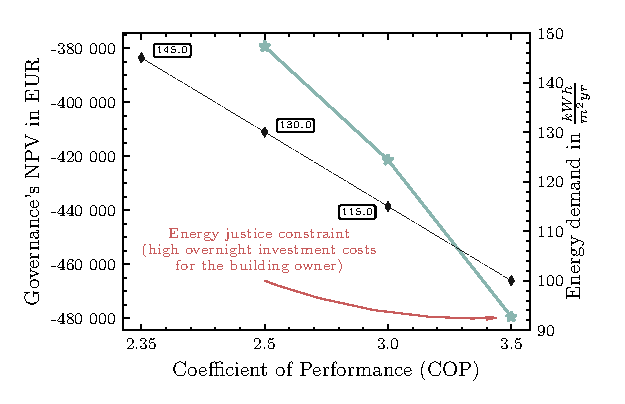
\includegraphics[width=0.75\linewidth]{figures/4_Results/fig_renovation_sens/renovation.eps}
	\caption{Justice-Constraint mit Sanierungskosten: Anstieg der Kosten sehr hoch.}
	\label{fig:cop1}
\end{figure}

FERNWÄRME UND WÄRMEPUMP FALL (DIRECTED TRANSITION UND SOCIETAL COMMITMENT) SENSITVITÄT AUFTEILUNG ZWISCHEN MIETER UND VERMIETER
% TODO Einpreisen der Mieterwechsel (Leerstand) in "Interest rate" des Landlords

% TODO Vergleich zwischen Government wo Gebäudesanierung voraussetzung ist und einmal ohne Gebäudesanierung - Demand seitige Anpassung
% TODO Gegenüberstellen: Einmal vergisst Staat auf Gebäudesanierung und einmal nicht, was ist das Delta an NPV. 

% TODO: Eventuell ist Modell dann nicht mehr Lösbar und was müsste die CO2 Aufteilung sein, damit es eine Lösung gibt. 